\documentclass[a4paper]{article}

%====================== PACKAGES ======================

\usepackage{etex}
\usepackage[french]{babel}
\usepackage[utf8x]{inputenc}
%pour gérer les positionnement d'images
\usepackage{float}
\usepackage{amsmath}
\usepackage{amssymb}
\usepackage{mathtools}
\usepackage{graphicx}
\usepackage[colorinlistoftodos]{todonotes}
\usepackage{url}
%pour les informations sur un document compilé en PDF et les liens externes / internes
\usepackage{hyperref}
%pour la mise en page des tableaux
\usepackage{array}
\usepackage{tabularx}
%pour utiliser \floatbarrier
%\usepackage{placeins}
%\usepackage{floatrow}
%espacement entre les lignes
\usepackage{setspace}
%modifier la mise en page de l'abstract
\usepackage{abstract}
%police et mise en page (marges) du document
\usepackage[T1]{fontenc}
\usepackage[top=2cm, bottom=2cm, left=2cm, right=2cm]{geometry}
%Pour les galerie d'images
\usepackage{subfig}
%landscape
\usepackage{pdflscape}
%pour l'algorithme
\usepackage{algorithmic}
\usepackage{algorithm2e}
%\usepackage{program}
\usepackage{listings}
\usepackage[parfill]{parskip}

%====================== INFORMATION ET REGLES ======================

%rajouter les numérotation pour les \paragraphe et \subparagraphe
% \setcounter{secnumdepth}{4}
% \setcounter{tocdepth}{4}

\hypersetup{							% Information sur le document
pdfauthor = {Guillaume Clochard
			Thomas Coquereau},			% Auteurs
pdftitle = {Mini-Projet d'Intelligence Artificielle
			Emploi du temps à Polytech Nantes},			% Titre du document
pdfsubject = {Compte Rendu Mini-Projet},		% Sujet
pdfkeywords = {},	% Mots-clefs
pdfstartview={FitH}}					% ajuste la page à la largueur de l'écran
%pdfcreator = {MikTeX},% Logiciel qui a crée le document
%pdfproducer = {}} % Société avec produit le logiciel

%======================== DEBUT DU DOCUMENT ========================

\begin{document}

% %régler l'espacement entre les lignes
% \newcommand{\HRule}{\rule{\linewidth}{0.5mm}}
% %espacement entre les lignes d'un tableau
% \renewcommand{\arraystretch}{1.5}

\title{Mini-Projet d'Intelligence Artificiel \\
    Emploi du temps à Polytech Nantes \\
    - \\
    Rapport complet}
\author{Guillaume Clochard, Thomas Coquereau}
\maketitle

% \tableofcontents

% \thispagestyle{empty}
% \setcounter{page}{0}
%ne pas numéroter le sommaire

%====================== INCLUSION DES PARTIES ======================

\section{Introduction}

Ce rapport présente un premier travail effectué dans le cadre du Mini-Projet
d'Intelligence Artificielle.
Il consiste en la planification de l'emploi du temps à Polytech Nantes.
Ce présent document contient le premier rendu (Résolution générale du problème),
ainsi que la suite du projet (Résolution du problème en Prolog).

Il est également fournit le code source du projet.


\begin{lstlisting}[language=bash, caption=Fichiers, captionpos=b]
README.md
instance.pl
instance_old.pl
main.pl
planifier.pl
run_test.pl
tests\
    instance.pl
    planifier.pl
    utils.pl
utils.pl
\end{lstlisting}

Le programme se lance par la commande suivante :

\begin{lstlisting}[language=bash, caption=Lancer l'algorithme, captionpos=b]
swipl -s main.pl
\end{lstlisting}

Les tests unitaires :

\begin{lstlisting}[language=bash, caption=Lancer les tests, captionpos=b]
swipl -s run_tests.pl
\end{lstlisting}

\newpage

\section{Résolution générale du problème}

\subsection{UML}

Voici dans la Figure \ref{fig:uml} le diagramme de classe décrivant les données
nécessaires à la gestion de l'emploi du temps.

Comme on peut le constater, on regroupe l'ensemble des données nécessaires et
déterminées à l'avance dans des Séances. A savoir : le(s) groupe(s) d'étudiants
concerné(s), le(s) enseignant(s), la matière, ainsi que le type de cours.
Ces séances vont ensuite être associées à des créneaux par notre solution.
Les créneaux étant le regroupement d'un jour, une plage horaire et une salle.

Un peu noter des détails intéressants, sur Groupe, il y a la notion
d'incompatibilité qui permet de définir lorsqu'il est possible pour deux groupes
d'avoir cours sur une même plage horaire. Sur matière on a la notion de suite,
lorsqu'une matière débute après la fin d'une autre (le Mini-Projet d'IA qui suit
par exemple le cours d'IA).
Et enfin sur séance, on a la notion de suite aussi qui décrit une nombre de
jours minimum et maximum avant le prochain cours de la même matière.

\textbf{Remarque}. Les noms données aux objets de la modélisation sont
légèrement différents de la solution donnée lors de l'indication de
mi-parcours. Nous appelons par exemple "Créneau" l'objet à construire et
regroupant Séance, Salle, Moment.

\begin{landscape}

    \begin{figure}[t]
        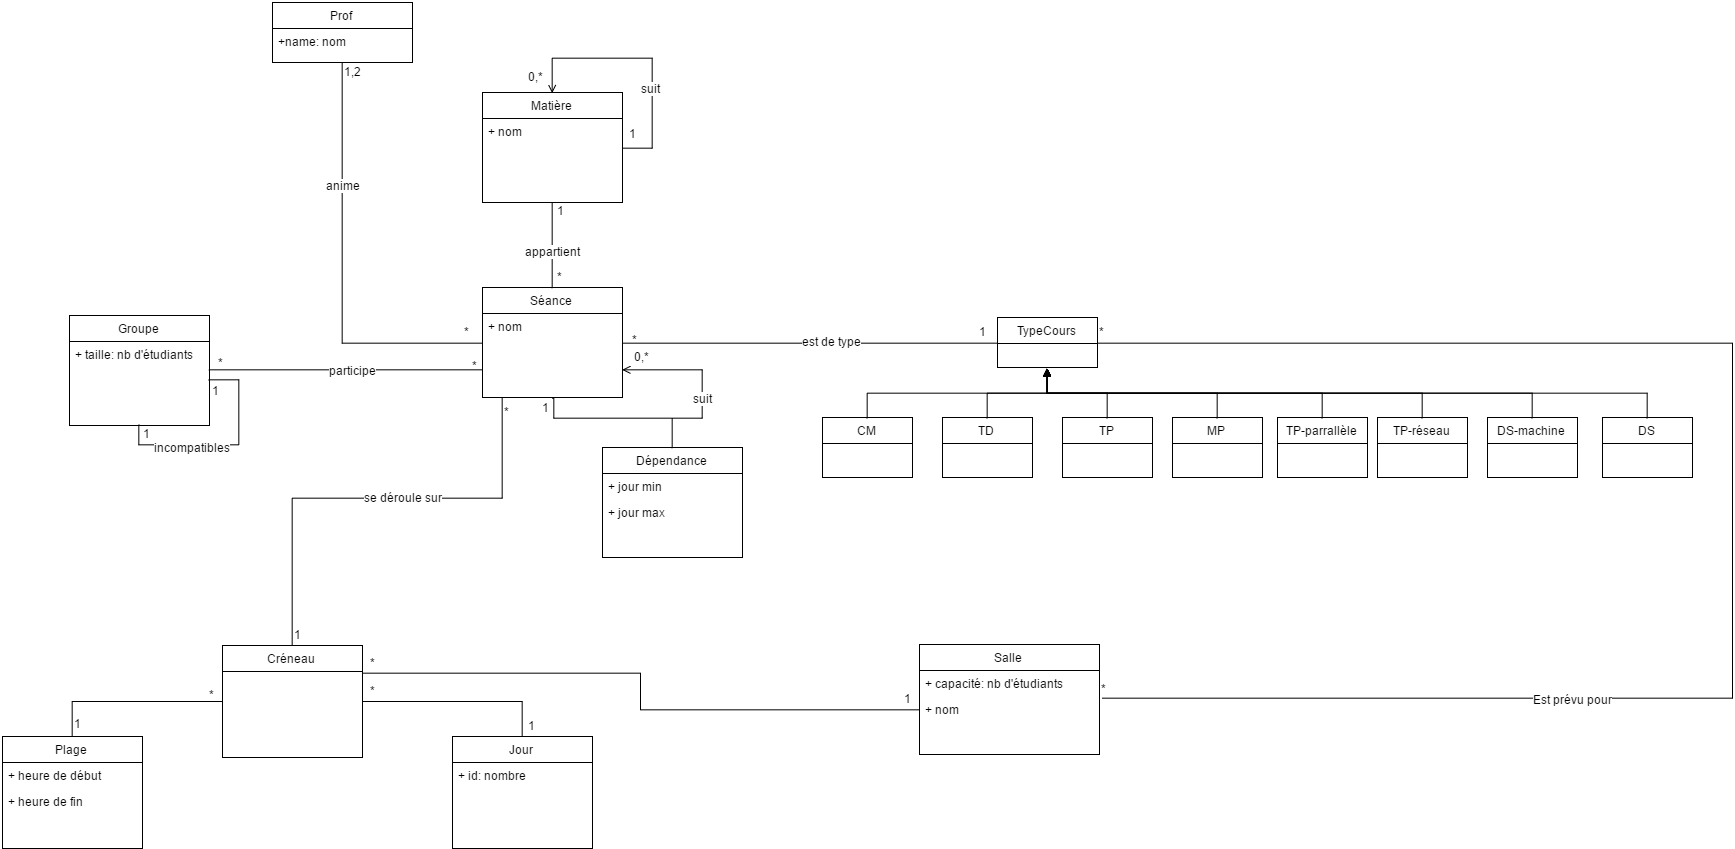
\includegraphics[keepaspectratio=true,width=26cm]{diagrammeClasse.png}
            \caption{\label{fig:uml} Modélisation UML}
    \end{figure}

\end{landscape}


\subsection{Instance}

Le problème modélisé, il convient maintenant de construire un jeu de données qui
servira à la construction de l'emploi du temps.

Deux instances sont disponibles :

\begin{description}

    \item[\texttt{instance\_old.pl}] Un petit jeu de données (17 séances) nous
        ayant servit au début du projet et servant actuellement pour les tests
        unitaires

    \item[\texttt{instance.pl}] Représente un semestre complet (458 séances,
        21 matières, 32 enseignants, 9 groupes, 20 salles)

\end{description}

Pour générer \texttt{instance.pl}, des prédicats ont été utilisés afin de
faciliter la saisie des données en regroupant les séances d'une même matière
dans une même déclaration.




\subsection{Solution}

Il convient à présent de définir une première proposition de solution.

Imaginons qu’on dispose d’une fonction $\textsc{Planifier}$ en charge de créer
l’emploi du temps.

Sa signature serait grossièrement :

\begin{description}

\item[Entrées] les séances $S$, les plages horaires $H$, les jours de
travail $J$, les mois $M$ et les salles $L$
\item[Sortie] un sous-ensemble de tous les créneaux $C$

\end{description}

\begin{center}

$\begin{array}{ll}
\textsc{Planifier} : S \times H \times J \times L \quad \not\to \quad C
\end{array}$

\end{center}

On retrouve donc les objets modélisés à la Figure \ref{fig:uml}.

\subsubsection{Pré-conditions}

Les pré-conditions de la fonction $\textsc{Planifier}$ sont formées par le respect
de la modélisations UML et de l'ajout de détails comme :

\begin{itemize}

    \item les jours sont des nombres entiers appartenant à $\mathbb{N}_{+}$
    \item les plages horaires ne débordent pas des 24h et ne se recouvrent pas

        \[
            \forall(h_0, h_1) \in H, h_0 \leq 0h00, h_1 \leq 23h59
        \]

        \[
            \forall(h_0, h_1),(h_2, h_3) \in H, \;
            h_0 < h_1 \leq h_2 < h_3 \;
            \text{ou} \; h_2 < h_3 \leq h_0 < h_1
        \]

    \item tous les types de cours des séances voient une salle compatible

        \[
            \forall s \in S, \exists l \in L, \text{typeCours}(s) =
            \text{typeCours}(l)
        \]

\end{itemize}

\subsubsection{Post-conditions}

\begin{itemize}

    \item les créneaux ne débordent pas sur des horaires, des jours ou des
        salles différents des entrés

        \begin{equation}\label{eqn:p1}
            \forall(s, h, j, l) \in \textsc{Planifier}(S, H, L, L),
            s \in S, h \in H, j \in J, l \in L
            \tag{P1}
        \end{equation}

    \item toutes les séances sont affectées à un créneau

        \begin{equation}\label{eqn:p2}
            \forall s \in S,
            \exists(s, h, j, l) \in \textsc{Planifier}(S, H, L, L)
            \tag{P2}
        \end{equation}

    \item toute séance est affectée à une salle qui respecte son type de cours
        et son effectif

        \begin{equation}\label{eqn:p3}
            \forall(s, h, j, l) \in \textsc{Planifier}(S, H, L, L),\;
            \text{typeCours}(s) = \text{typeCours}(l)
            \  \text{et} \  \text{effectif}(s) \leq \text{taille}(l)
            \tag{P3}
        \end{equation}

    \item un enseignant n'a pas deux séances en même temps

        \begin{equation}\label{eqn:p4}
            \forall(s_1, h, j, l_1), (s_2, h, j, l_2)
            \in \textsc{Planifier}(S, H, L, L),\;
            \text{prof}(s_1) \not= \text{prof}(s_2)
            \tag{P4}
        \end{equation}

    \item des groupes incompatibles n'ont pas cours en même temps

        \begin{equation}\label{eqn:p5}
            \begin{split}
                & \forall(s_1, h, j, l_1), (s_2, h, j, l_2)
                \in \textsc{Planifier}(S, H, L, L),\;\\
                & \lnot\text{incompatibles}(g_1, g_2)
                \quad \forall g_1 \in groupes(s_1), \forall g_2 \in groupes(s_2)
            \end{split}
            \tag{P5}
        \end{equation}

    \item les créneaux respectent le séquencement des séances et des matières

        \begin{equation}\label{eqn:p6}
            \begin{split}
                & \forall(s_1, h_1, j_1, l_1), (s_2, h_2, j_2, l_2)
                \in \textsc{Planifier}(S, H, L, L),
                \text{tel que} \  \text{suit}(s_2, s_1)\\
                & \text{alors} \  j_2 \in O
                \  \text{où} \  O = intervalleJours(s_1, s_2)\\
                & \text{et si} \  j_2 = j_1 \  \text{alors} \  h_2 > h_1
            \end{split}
            \tag{P6}
        \end{equation}

\end{itemize}


\subsubsection{Algorithme non déterministe}

Nous avons choisit de formuler notre solution sous forme d'un algorithme non
déterministe.

Dans l'algorithme \ref{algo:algo1}, on construit des créneaux liant correctement
une séance, un horaire, un jour ainsi qu'une salle à l'aide de l'\emph{oracle}
\texttt{choix\_nd}.

À chaque nouveau choix, on teste si les post-conditions $P_i$ données au-dessus
sont respectées.
Si c'est le cas, on ajoute le créneau composé de ces données
dans la liste des créneaux et on enlève la séance de la liste des séance.
Si ces les post-conditions ne sont pas respectées par le nouvel ajout, on
retourne $\perp$ afin de marquer l'échec de ce créneau.

On continue ainsi jusqu'à ce qu'il n'y ait plus de séances à placer.

\begin{algorithm}
\caption{Proposition de solution}
\label{algo:algo1}
\begin{algorithmic}
    \STATE $C \Leftarrow \emptyset$
    \WHILE{$|S| > 0$}
        \STATE $s \Leftarrow choix\_nd(S)$
        \STATE $h \Leftarrow choix\_nd(H)$
        \STATE $j \Leftarrow choix\_nd(J)$
        \STATE $l \Leftarrow choix\_nd(L)$
        \STATE $c \Leftarrow (s, h, j, l)$
        \IF{les post-conditions $P_i$ sont respectées avec $c$}
            \STATE $C \Leftarrow c \cup C$
            \STATE $S \Leftarrow S \backslash s$
        \ELSE
            \RETURN $\perp$
        \ENDIF
    \ENDWHILE
\end{algorithmic}
\end{algorithm}




\newpage

\section{Résolution du problème en Prolog}


\subsection{Algorithme}

\subsubsection{Résolution}

\begin{lstlisting}[language=Prolog, caption=Resolution, captionpos=b]
/**
 * planifier(+Ss, -Cs).
 *
 * @arg S   Listes des séances à planifier
 * @arg C   Listes des créneaux construits
 */
planifier([], []) :- !.
planifier(Ss, [C|Cs]) :-

    member(S, Ss),      % La séance courante
    delete(Ss, S, Ss2), % On l'enlève de la liste

    planifier(Ss2, Cs), % on traite le sous-problème

    % Création du créneau et tests ---------------------------------------------

    seance(S, TypeS, _, _),

    date(J, M),     % une date
    plage(H, _, _), % une plage horaire

    % une salle
    salle(L, TailleL),
    accueille(L, TypeL),
    typesCoursIdentiques(TypeS, TypeL), % type de salle valide

    findall(G, groupeSeance(G, S), Gs), % tous les groupes de la séance
    effectifGroupes(Gs, Effectif),
    Effectif =< TailleL, % taille de salle valide

    findall(P, profSeance(P, S), Ps),   % tous les enseignants de la séance

    % test des contraintes (profs, incompatibilité groupes, séquencement)
    % sur cette proposition de créneau
    creneauValide(S, Ps, Gs, H, J, M, L, Cs),

    % Fin création du créneau et tests -----------------------------------------

    C = [S, H, J, M, L].
\end{lstlisting}

Voici, dans le code ci-dessus, notre fonction de résolution "planifier(Ss, Cs)". 

Nous avons essayé d'écrire un code qui soit \emph{atomique} au maximum. Chaque fonction effectue une action précise, ou bien est ensuite divisée en plusieurs fonctions qui elles effectueront des requêtes atomiques.

Après avoir récupéré la séance courante, on traite ce sous problème. 
On cherche à diviser le problème pour qu'il traite chaque séance indépendamment. 

Une fois que l'on s'attaque à une seule séance. On va faire les \emph{choix\_nd} décris dans l'algorithme \ref{algo:algo1}.

L'ordre de ces choix est important car la récursivité de Prolog remontera et trouvera de nouvelles valeurs dans l'ordre que nous avons défini.

Tout d'abord, on détermine la date ainsi que la plage horaire via deux \emph{choix\_nd}. 
On commence par ces choix-ci car cela permet de s'assurer que l'on aura les cours sur des créneaux similaires. 
Exemples : le 01/01, de 14h à 15h30, on peut avoir plusieurs séances avec des groupes différents et des salles différentes.

En effet auparavan nous commencions par déterminer la salle et l'emploi du temps était beaucoup plus étendu car les créneaux ne se superposaient que très peu.

Dans un second temps, on va donc trouver une salle qui peut accueillir suffisamment d'élèves ainsi que le bon type de cours. Tant que ces deux variables ne sont pas vraies, Prolog va effectuer un \emph{choix\_nd} de salle.

Ensuite on se penche sur les problèmes de groupes. 
On récupère les groupes associés à la séance, et on vérifie qu'ils ne sont pas trop nombreux par rapport à la salle choisie. 
Si c'est le cas, Prolog va remonter à la fonction précédente, c'est à dire le choix de la salle. 

Il est donc important dans ce cas de les effectuer l'une après l'autre.

Après cela, on récupère le(s) professeur(s) associé(s) à la séance.

Cet ordre permet que, pour un même créneau, on regarde toutes les salles qui correspondent avant de changer de créneau. C'est une bonne façon de régler le problème d'avoir des cours en parallèles.

\subsubsection{Prédicats utilitaires}

\begin{lstlisting}[language=Prolog, caption=creneauValide, captionpos=b]
/**
 * creneauValide(S, Ps, G, H, J, M, L, [Cs]).
 *
 * Définit si un creneau est valide (Pas de conflit avec les créneaux existants)
 *
 * @arg S   La séance
 * @arg Ps  Les enseignants
 * @arg Gs  Les groupes
 * @arg H   La plage horaire
 * @arg J   Le jour
 * @arg M   Le mois
 * @arg L   La salle
 * @arg Cs  Liste de créneaux [S, H, J, M, L]
 */
creneauValide(_, _, _, _, _, _, _, []) :- !.
creneauValide(S, Ps, Gs, H, J, M, L, [C|Cs]) :-
    creneauValideCreneau(S, Ps, Gs, H, J, M, L, C),
    creneauValide(S, Ps, Gs, H, J, M, L, Cs),
    !.
\end{lstlisting}

TODO décrire ce qui se passe dans \texttt{creneauValide} et les prédicats
utilisés (mettre leur signature, pas le code)






\subsection{Ordonnancement et heuristique}

Il est important de remarquer que les séances peuvent être ordonnées avant de
chercher une planification. Les séances d'une même matière se suivant, il est
intéressant de commencer par planifier la première, puis la seconde, etc.

Le prédicat \texttt{indiceSeance(+S, -I)} implémente donc l'heuristique
retournant l'indice d'une séance dans l'arbre des séances séquencées. Cette
heuristique nous permet de trier les séances à priori et de commencer la
la planification des séances de plus petits indices. Elles doivent logiquement
se dérouler en début de période scolaire.

Cet ordonnancement nous permet de rapidement partir dans une branche
relativement bonne. Sans ordonnancement, on peut trouver le moteur d'inférence
ayant commencé par placer la dernière séance d'une matière sur le premier
créneau de l'année, ce qui entraine alors de très nombreux retours arrières.




\subsection{Performances}

Les performances de l'algorithme final sur notre jeu de données complet (458 séances,
21 matières, 32 enseignants, 9 groupes, 20 salles) peuvent être capturées avec
\texttt{profile(planification(Cs))}.

Le résultat est à la figure \ref{fig:profile}.

On remarque donc un temps de 1,68 secondes sur une machine donnée. Les
performances peuvent être améliorées encore, on le voit, en réduisant l'usage du
prédicat \texttt{member/2}. C'est par exemple notre prédicat
\texttt{accueille(+Salle, ?TypeCours)}, très utilisé, qui en fait un usage
important. Cette donnée pourrait être déclaré au lancement du programme par
\texttt{assert/1}.

\begin{figure}[H]
	\centering
    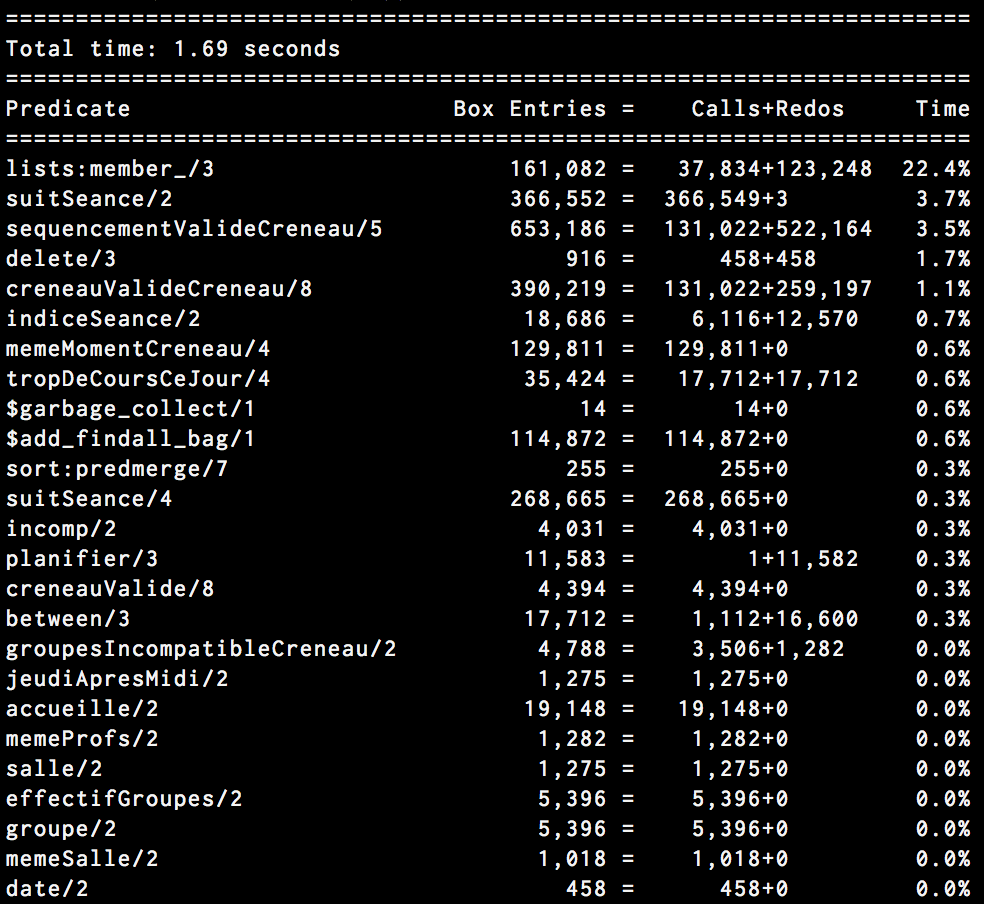
\includegraphics[keepaspectratio=true,width=12cm]{profile.png}
        \caption{\label{fig:profile} Résultat du profiling }
\end{figure}



\subsection{\textit{One more thing}}

TODO parler de l'affichage

TODO parler des prédicats supplémentaires pour optimiser l'emploi du temps

TODO parler des tests




\newpage

\section{Conclusion}



\end{document}
